\section{Software design}
some general info

\subsection{Peripherals} %please think about the appropriate name!
The description of our modular architecture, the work principles of the separate modules and basically "how we control the peripherals" such as motors, leds, timers, etc. Logic comes a bit later in here.
Also all info on DMA and pin remapping and our pretty mapping table are also welcomed here I think

\subsubsection*{Timer 1}
Short description on how we worked out the time

\subsubsection*{Pulse Width Modulation (PWM)}

\begin{figure}[htb]
    \centering
    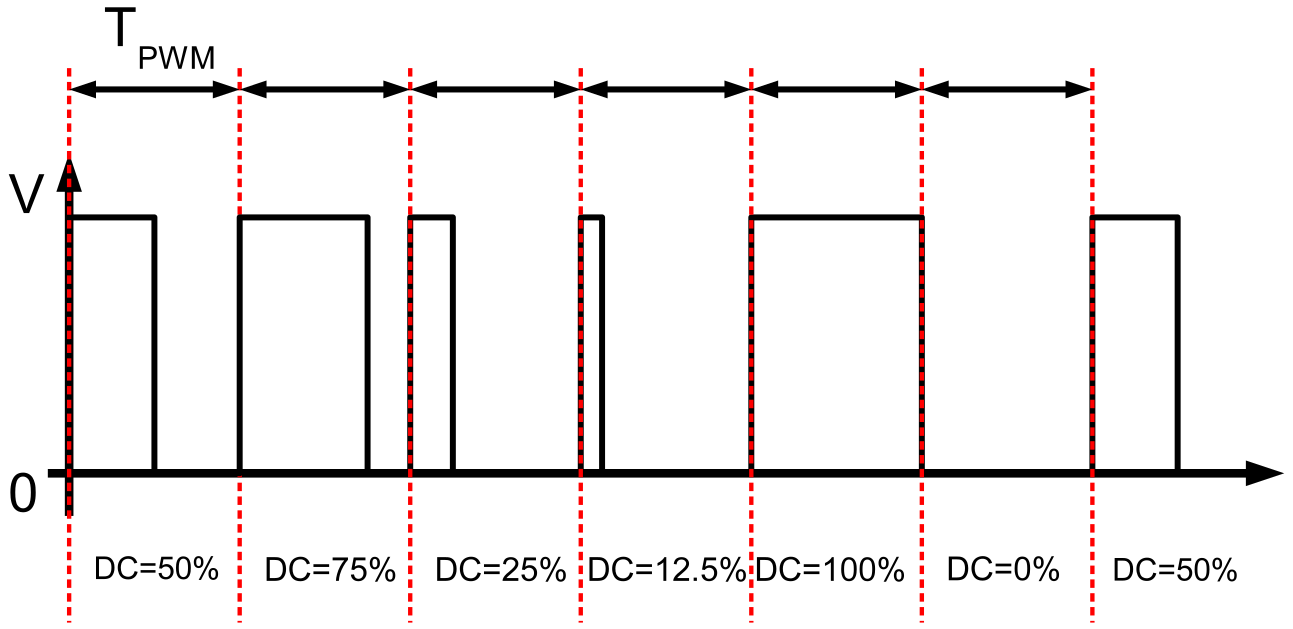
\includegraphics[width=0.6\textwidth]{figures/software/pwm_demo.png}
    \caption {Principle of PWM \cite{alex}}
    \label{fig:pwm_demo}
\end{figure}

Pulse Width Modulation allows us to control the amount of energy supplied to an actuator. In this case we use the PWM signal to drive our motors and control their speed. Using different pulse widths, we can supply different amount of power to our motors. \cite{alex}


As seen in figure \ref{fig:pwm_demo}, we have a fixed PWM period $T_{PWM}$. We can now vary the so called duty cycle $DC$ by changing the time the PWM output is switched on ($T_{DC}$).
\begin{equation}
    DC = \frac{T_{DC}}{T_{PWM}}
\end{equation}
For our PWM unit, we mainly have to choose the parameters:
\begin{enumerate}
    \item PWM period
    \item PWM duty cycle
\end{enumerate}


Depending on our PWM period, we get different amount of ripple in our resulting signal. More on this can be found in \cite[Chapter~5.1]{alex}. In figure \ref{fig:pwm_choice} is an example of possible choices for the PWM period register ($PTPER$) and the PWM duty cycle register ($PDC$)

\begin{figure}[htb]
    \centering
    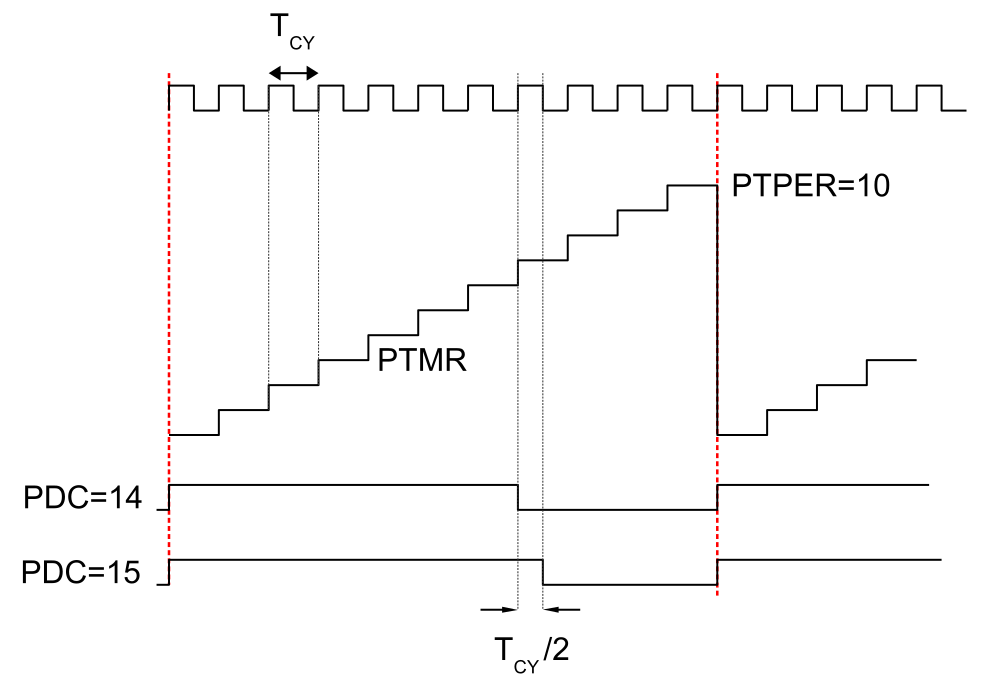
\includegraphics[width=0.6\textwidth]{figures/software/pwm_choice.png}
    \caption {Example: Resolution of PWM duty cycle \cite{alex}}
    \label{fig:pwm_choice}
\end{figure}

For our motors, we have the following parameters:
\begin{itemize}
    \item \textbf{fixed}: $T_{CY} = 25 ns$
    \item timer prescaler $PTCKPS = 0b00$ (option 1:1)
    \item PWM period register $P1TPER = 2000 - 1$
    \item PWM duty cycle $PDC \in [0, 2*(P1TPER + 1)]$
\end{itemize}
$T_{PWM} = ( PTPER + 1 ) * T_{CY} = 2000 * 20ns = 40000 ns$


$f_{PWM} = \frac{1}{T_{PWM}} = 0.25 * 10^{5} Hz$

With the current values, we can now set different duty cycles for our motors by choosing valid values for the $PDC$ register.


\subsubsection*{Quadrature Encoder Inferface(QEI)}
how does qei work?

\subsubsection*{Analogue-to-Digital Conversion(ADC)}

\subsubsection*{Direct Memory Access (DMA) - does this belong here?}

\subsubsection*{Universal Asynchronous Receiver Transmitter (UART)}


\subsection{Pin Mapping}
maybe a diagram of which peripheral maps to which pin


\subsection{Controller Design and Approach}

Here goes the whole logic of the mouse movement control (how should it behave when is faced with the wall or on contrary - with the gap in the labyrinth). PID controller design and the logic behind it.

\subsubsection{Proportional-Integral-Derivative Controller (PID)}

\subsubsection{State Machine}



